\documentclass{standalone}
\usepackage{tikz}
\usetikzlibrary{patterns, positioning}


\begin{document}
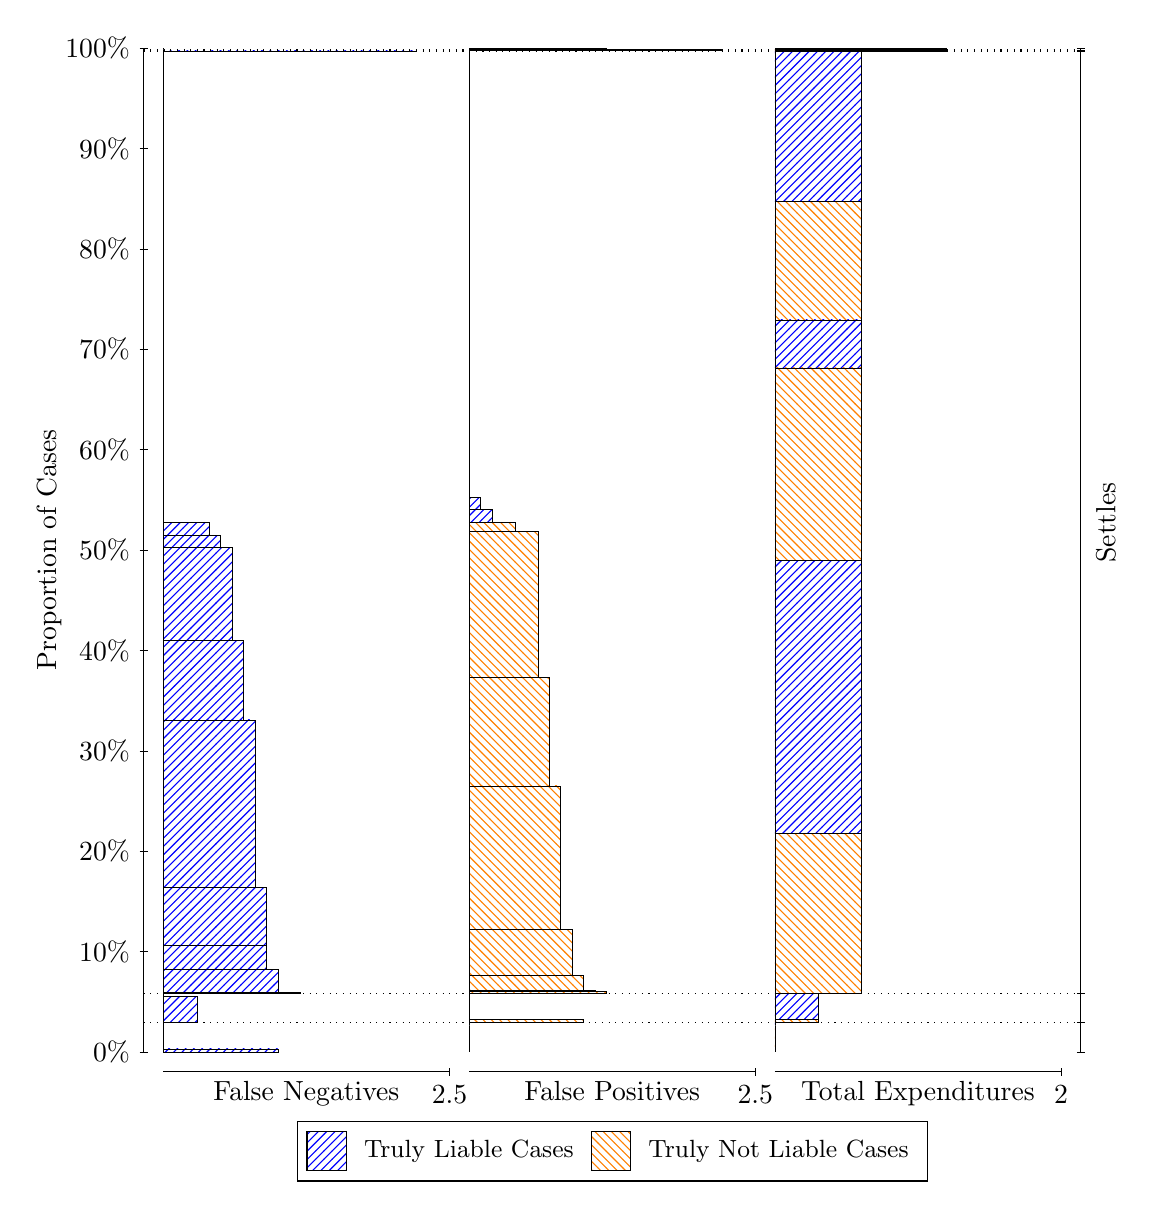
\begin{tikzpicture}
\draw[black, very thin] (1.5,1.75) -- (1.5,14.5);
\node[rotate=90, text=black, anchor=center] at (0.3, 8.125) {Proportion of Cases};
\draw[black, very thin] (1.45,1.75) -- (1.55,1.75);
\node[text=black, anchor=east] at (1.45, 1.75) {0\%};
\draw[black, very thin] (1.45,3.025) -- (1.55,3.025);
\node[text=black, anchor=east] at (1.45, 3.025) {10\%};
\draw[black, very thin] (1.45,4.3) -- (1.55,4.3);
\node[text=black, anchor=east] at (1.45, 4.3) {20\%};
\draw[black, very thin] (1.45,5.575) -- (1.55,5.575);
\node[text=black, anchor=east] at (1.45, 5.575) {30\%};
\draw[black, very thin] (1.45,6.85) -- (1.55,6.85);
\node[text=black, anchor=east] at (1.45, 6.85) {40\%};
\draw[black, very thin] (1.45,8.125) -- (1.55,8.125);
\node[text=black, anchor=east] at (1.45, 8.125) {50\%};
\draw[black, very thin] (1.45,9.4) -- (1.55,9.4);
\node[text=black, anchor=east] at (1.45, 9.4) {60\%};
\draw[black, very thin] (1.45,10.675) -- (1.55,10.675);
\node[text=black, anchor=east] at (1.45, 10.675) {70\%};
\draw[black, very thin] (1.45,11.95) -- (1.55,11.95);
\node[text=black, anchor=east] at (1.45, 11.95) {80\%};
\draw[black, very thin] (1.45,13.225) -- (1.55,13.225);
\node[text=black, anchor=east] at (1.45, 13.225) {90\%};
\draw[black, very thin] (1.45,14.5) -- (1.55,14.5);
\node[text=black, anchor=east] at (1.45, 14.5) {100\%};

\draw[black, very thin] (13.4,1.75) -- (13.4,14.5);
\draw[black, very thin] (13.35,1.75) -- (13.45,1.75);
\node[anchor=west] at (13.35, 1.75) {};
\draw[black, very thin] (13.35,2.1226) -- (13.45,2.1226);
\node[anchor=west] at (13.35, 2.1226) {};
\draw[black, very thin] (13.35,2.4953) -- (13.45,2.4953);
\node[anchor=west] at (13.35, 2.4953) {};
\draw[black, very thin] (13.35,14.456) -- (13.45,14.456);
\node[anchor=west] at (13.35, 14.456) {};
\draw[black, very thin] (13.35,14.475) -- (13.45,14.475);
\node[anchor=west] at (13.35, 14.475) {};
\draw[black, very thin] (13.35,14.5) -- (13.45,14.5);
\node[anchor=west] at (13.35, 14.5) {};

\draw[black, very thin, pattern color=blue, pattern=north east lines] (1.75,1.75) rectangle (3.2033,1.7892);
\draw[black, very thin, pattern color=orange, pattern=north west lines] (1.75,1.7892) rectangle (1.75,2.1226);
\draw[black, very thin, pattern color=blue, pattern=north east lines] (1.75,2.1226) rectangle (2.186,2.4561);
\draw[black, very thin, pattern color=orange, pattern=north west lines] (1.75,2.4561) rectangle (1.75,2.4953);
\draw[black, very thin, pattern color=blue, pattern=north east lines] (1.75,2.4953) rectangle (3.494,2.5103);
\draw[black, very thin, pattern color=blue, pattern=north east lines] (1.75,2.5103) rectangle (3.2033,2.7973);
\draw[black, very thin, pattern color=blue, pattern=north east lines] (1.75,2.7973) rectangle (3.058,3.1046);
\draw[black, very thin, pattern color=blue, pattern=north east lines] (1.75,3.1046) rectangle (3.058,3.8385);
\draw[black, very thin, pattern color=blue, pattern=north east lines] (1.75,3.8385) rectangle (2.9127,5.9684);
\draw[black, very thin, pattern color=blue, pattern=north east lines] (1.75,5.9684) rectangle (2.7673,6.9755);
\draw[black, very thin, pattern color=blue, pattern=north east lines] (1.75,6.9755) rectangle (2.622,8.1624);
\draw[black, very thin, pattern color=blue, pattern=north east lines] (1.75,8.1624) rectangle (2.4767,8.3125);
\draw[black, very thin, pattern color=blue, pattern=north east lines] (1.75,8.3125) rectangle (2.3313,8.4725);
\draw[black, very thin, pattern color=orange, pattern=north west lines] (1.75,8.4725) rectangle (1.75,14.456);
\draw[black, very thin, pattern color=blue, pattern=north east lines] (1.75,14.456) rectangle (4.9473,14.463);
\draw[black, very thin, pattern color=orange, pattern=north west lines] (1.75,14.463) rectangle (1.75,14.475);
\draw[black, very thin, pattern color=orange, pattern=north west lines] (1.75,14.475) rectangle (1.75,14.482);
\draw[black, very thin, pattern color=blue, pattern=north east lines] (1.75,14.482) rectangle (1.75,14.5);
\draw[black, very thin, pattern color=orange, pattern=north west lines] (5.6333,1.75) rectangle (5.6333,2.0834);
\draw[black, very thin, pattern color=blue, pattern=north east lines] (5.6333,2.0834) rectangle (5.6333,2.1226);
\draw[black, very thin, pattern color=orange, pattern=north west lines] (5.6333,2.1226) rectangle (7.0867,2.1618);
\draw[black, very thin, pattern color=blue, pattern=north east lines] (5.6333,2.1618) rectangle (5.6333,2.4953);
\draw[black, very thin, pattern color=orange, pattern=north west lines] (5.6333,2.4953) rectangle (7.3773,2.5149);
\draw[black, very thin, pattern color=orange, pattern=north west lines] (5.6333,2.5149) rectangle (7.232,2.5298);
\draw[black, very thin, pattern color=orange, pattern=north west lines] (5.6333,2.5298) rectangle (7.0867,2.7227);
\draw[black, very thin, pattern color=orange, pattern=north west lines] (5.6333,2.7227) rectangle (6.9413,3.3035);
\draw[black, very thin, pattern color=orange, pattern=north west lines] (5.6333,3.3035) rectangle (6.796,5.1299);
\draw[black, very thin, pattern color=orange, pattern=north west lines] (5.6333,5.1299) rectangle (6.6507,6.5082);
\draw[black, very thin, pattern color=orange, pattern=north west lines] (5.6333,6.5082) rectangle (6.5053,8.3655);
\draw[black, very thin, pattern color=orange, pattern=north west lines] (5.6333,8.3655) rectangle (6.2147,8.4784);
\draw[black, very thin, pattern color=blue, pattern=north east lines] (5.6333,8.4784) rectangle (5.924,8.6384);
\draw[black, very thin, pattern color=blue, pattern=north east lines] (5.6333,8.6384) rectangle (5.7787,8.7885);
\draw[black, very thin, pattern color=blue, pattern=north east lines] (5.6333,8.7885) rectangle (5.6333,14.456);
\draw[black, very thin, pattern color=orange, pattern=north west lines] (5.6333,14.456) rectangle (5.6333,14.468);
\draw[black, very thin, pattern color=blue, pattern=north east lines] (5.6333,14.468) rectangle (5.6333,14.475);
\draw[black, very thin, pattern color=orange, pattern=north west lines] (5.6333,14.475) rectangle (8.8307,14.482);
\draw[black, very thin, pattern color=blue, pattern=north east lines] (5.6333,14.482) rectangle (7.3773,14.5);
\draw[black, very thin, pattern color=orange, pattern=north west lines] (9.5167,1.75) rectangle (9.5167,2.0834);
\draw[black, very thin, pattern color=blue, pattern=north east lines] (9.5167,2.0834) rectangle (9.5167,2.1226);
\draw[black, very thin, pattern color=orange, pattern=north west lines] (9.5167,2.1226) rectangle (10.062,2.1618);
\draw[black, very thin, pattern color=blue, pattern=north east lines] (9.5167,2.1618) rectangle (10.062,2.4953);
\draw[black, very thin, pattern color=orange, pattern=north west lines] (9.5167,2.4953) rectangle (10.607,4.5293);
\draw[black, very thin, pattern color=blue, pattern=north east lines] (9.5167,4.5293) rectangle (10.607,7.9963);
\draw[black, very thin, pattern color=orange, pattern=north west lines] (9.5167,7.9963) rectangle (10.607,10.437);
\draw[black, very thin, pattern color=blue, pattern=north east lines] (9.5167,10.437) rectangle (10.607,11.046);
\draw[black, very thin, pattern color=orange, pattern=north west lines] (9.5167,11.046) rectangle (10.607,12.555);
\draw[black, very thin, pattern color=blue, pattern=north east lines] (9.5167,12.555) rectangle (10.607,14.456);
\draw[black, very thin, pattern color=orange, pattern=north west lines] (9.5167,14.456) rectangle (11.697,14.468);
\draw[black, very thin, pattern color=blue, pattern=north east lines] (9.5167,14.468) rectangle (11.697,14.475);
\draw[black, very thin, pattern color=orange, pattern=north west lines] (9.5167,14.475) rectangle (11.697,14.482);
\draw[black, very thin, pattern color=blue, pattern=north east lines] (9.5167,14.482) rectangle (11.697,14.5);
\draw[black, dotted] (1.5,2.1226) -- (13.4,2.1226);
\draw[black, dotted] (1.5,2.4953) -- (13.4,2.4953);
\draw[black, dotted] (1.5,14.456) -- (13.4,14.456);
\draw[black, dotted] (1.5,14.475) -- (13.4,14.475);
\draw[black, very thin] (1.75,1.5) -- (5.3833,1.5);
\node[text=black, anchor=north] at (3.5667, 1.5) {False Negatives};
\draw[black, very thin] (5.3833,1.45) -- (5.3833,1.55);
\node[text=black, anchor=north] at (5.3833, 1.45) {2.5};

\draw[black, very thin] (5.6333,1.5) -- (9.2667,1.5);
\node[text=black, anchor=north] at (7.45, 1.5) {False Positives};
\draw[black, very thin] (9.2667,1.45) -- (9.2667,1.55);
\node[text=black, anchor=north] at (9.2667, 1.45) {2.5};

\draw[black, very thin] (9.5167,1.5) -- (13.15,1.5);
\node[text=black, anchor=north] at (11.333, 1.5) {Total Expenditures};
\draw[black, very thin] (13.15,1.45) -- (13.15,1.55);
\node[text=black, anchor=north] at (13.15, 1.45) {2};



\node[text=black, centered, rotate=90] at (13.72, 8.4755) {Settles};



\draw (7.449999999999999,1.5) node[draw=none] (baseCoordinate) {};
\begin{scope}[align=center]
        \matrix[scale=0.5, draw=black, below=0.5cm of baseCoordinate, nodes={draw}, column sep=0.1cm]{
            \node[rectangle, draw, minimum width=0.5cm, minimum height=0.5cm, pattern color=blue, pattern=north east lines] {}; &
            \node[draw=none, font=\small, text=black] (B) {Truly Liable Cases}; &
            \node[rectangle, draw, minimum width=0.5cm, minimum height=0.5cm, pattern color=orange, pattern=north west lines] {}; &
            \node[draw=none, font=\small, text=black] (B) {Truly Not Liable Cases}; \\
            };
\end{scope}

\end{tikzpicture}
\end{document}